% CS669: Pattern Recognition
% Programming Assignment I
% Gabriel Dulac-Arnold <gabe@squirrelsoup.net>
% Johannes H. Jensen <johannj@stud.ntnu.no>
\documentclass[a4paper]{article}
\usepackage{multicol}
\usepackage{graphicx}
\usepackage[top=2cm,nohead,nofoot]{geometry}

\author{Gabriel Dulac-Arnold $<$gabe@squirrelsoup.net$>$ (CS09F004) \\
Johannes H. Jensen $<$johannj@stud.ntnu.no$>$ (CS09F005) \\
\\
(Batch no. 14)}
\title{CS669 - Pattern Recognition\\
\emph{Programming Assignment 1}}

\begin{document}
\setlength{\parskip}{2ex}
\maketitle

\section{Classifier Accuracy for Each Dataset}

\begin{tabular}{ l | c | c | c | c | c | }
Dataset & B $C_{mean}$ & B $C_{distinct}$ & NB $\sigma^2 I$ & NB $C_{mean}$ & NB $C_{distinct}$\\
\hline
  LS & 99.73\% & 100\% & 99.73\% & 99.73\% & 99.73\% \\ 
\hline
  NLS & 62.17\% & 62.01\% & 62.58\% & 62.42\% & 62.58\% \\
\hline
  OL & 88.53\% & 92.54\% & 88.00\% & 88.53\% & 89.07\% \\
\hline
  RL & 77.61\% & 77.44\% & 77.20\% & 77.43\% & 77.43\% \\
\hline
\end{tabular}

\section{Confusion Matrices}
\begin{enumerate}
\item Bayes $C_{mean}$

\begin{multicols}{2}
\begin{enumerate}
\item Linearly Seperable

\begin{tabular}{ l | c | c | c | }

& $\omega_1$ & $\omega_2$ & $\omega_3$ \\
\hline
  $\omega_1$ & 124 & 1 & 0 \\ 
\hline
  $\omega_2$ & 0 & 125 & 0 \\
\hline
  $\omega_3$ & 0 & 0 & 125 \\
\hline
\end{tabular}


\item Non-Linearly Seperable

\begin{tabular}{ l | c | c |}

& $\omega_1$ & $\omega_2$ \\
\hline
  $\omega_1$ & 384 & 228 \\ 
\hline
  $\omega_2$ & 235 & 377 \\
\hline
\end{tabular}
\newline

\item Overlapping Data

\begin{tabular}{ l | c | c | c | }
& $\omega_1$ & $\omega_2$ & $\omega_3$ \\
\hline
  $\omega_1$ & 106 & 17 & 2 \\ 
\hline
  $\omega_2$ & 0 & 109 & 16 \\
\hline
  $\omega_3$ & 7 & 1 & 117 \\
\hline
\end{tabular}

\item Real World Data

\begin{tabular}{ l | c | c | c | }
& $\omega_1$ & $\omega_2$ & $\omega_3$ \\
\hline
  $\omega_1$ & 571 & 23 & 3 \\ 
\hline
  $\omega_2$ & 343 & 213 & 17 \\
\hline
  $\omega_3$ & 0 & 0 & 622 \\
\hline
\end{tabular}
\end{enumerate}
\end{multicols}

\item Bayes $C_{distinct}$

\begin{multicols}{2}
\begin{enumerate}
\item Linearly Seperable

\begin{tabular}{ l | c | c | c | }

& $\omega_1$ & $\omega_2$ & $\omega_3$ \\
\hline
  $\omega_1$ & 125 & 0 & 0 \\ 
\hline
  $\omega_2$ & 0 & 125 & 0 \\
\hline
  $\omega_3$ & 0 & 0 & 125 \\
\hline
\end{tabular}

\item Non-Linearly Seperable

\begin{tabular}{ l | c | c |}

& $\omega_1$ & $\omega_2$ \\
\hline
  $\omega_1$ & 379 & 233 \\ 
\hline
  $\omega_2$ & 232 & 380 \\
\hline
\end{tabular}
\newline

\item Overlapping Data

\begin{tabular}{ l | c | c | c | }

& $\omega_1$ & $\omega_2$ & $\omega_3$ \\
\hline
  $\omega_1$ & 114 & 8 & 3 \\ 
\hline
  $\omega_2$ & 4 & 116 & 5 \\
\hline
  $\omega_3$ & 6 & 2 & 117 \\
\hline
\end{tabular}

\item Real World Data

\begin{tabular}{ l | c | c | c | }
& $\omega_1$ & $\omega_2$ & $\omega_3$ \\
\hline
  $\omega_1$ & 571 & 23 & 3 \\ 
\hline
  $\omega_2$ & 343 & 211 & 15 \\
\hline
  $\omega_3$ & 0 & 1 & 621 \\
\hline
\end{tabular}
\end{enumerate}
\end{multicols}

\newpage

\item Naive Bayes $C = \sigma^2I$
\begin{multicols}{2}
\begin{enumerate}
\item Linearly Seperable

\begin{tabular}{ l | c | c | c | }

& $\omega_1$ & $\omega_2$ & $\omega_3$ \\
\hline
  $\omega_1$ & 124 & 1 & 0 \\ 
\hline
  $\omega_2$ & 0 & 125 & 0 \\
\hline
  $\omega_3$ & 0 & 0 & 125 \\
\hline
\end{tabular}

\item Non-Linearly Seperable

\begin{tabular}{ l | c | c |}

& $\omega_1$ & $\omega_2$ \\
\hline
  $\omega_1$ & 388 & 224 \\ 
\hline
  $\omega_2$ & 234 & 378 \\
\hline
\end{tabular}
\newline

\item Overlapping Data

\begin{tabular}{ l | c | c | c | }

& $\omega_1$ & $\omega_2$ & $\omega_3$ \\
\hline
  $\omega_1$ & 106 & 17 & 2 \\ 
\hline
  $\omega_2$ & 2 & 106 & 17 \\
\hline
  $\omega_3$ & 6 & 1 & 118 \\
\hline
\end{tabular}

\item Real World Data

\begin{tabular}{ l | c | c | c | }
& $\omega_1$ & $\omega_2$ & $\omega_3$ \\
\hline
  $\omega_1$ & 570 & 24 & 3 \\ 
\hline
  $\omega_2$ & 348 & 207 & 18 \\
\hline
  $\omega_3$ & 0 & 0 & 622 \\
\hline
\end{tabular}
\end{enumerate}
\end{multicols}

\item Naive Bayes $C_{mean}$
\begin{multicols}{2}
\begin{enumerate}
\item Linearly Seperable

\begin{tabular}{ l | c | c | c | }
& $\omega_1$ & $\omega_2$ & $\omega_3$ \\
\hline
  $\omega_1$ & 124 & 1 & 0 \\ 
\hline
  $\omega_2$ & 0 & 125 & 0 \\
\hline
  $\omega_3$ & 0 & 0 & 125 \\
\hline
\end{tabular}

\item Non-Linearly Seperable

\begin{tabular}{ l | c | c |}

& $\omega_1$ & $\omega_2$ \\
\hline
  $\omega_1$ & 386 & 226 \\ 
\hline
  $\omega_2$ & 234 & 378 \\
\hline
\end{tabular}
\newline

\item Overlapping Data

\begin{tabular}{ l | c | c | c | }

& $\omega_1$ & $\omega_2$ & $\omega_3$ \\
\hline
  $\omega_1$ & 106 & 17 & 2 \\ 
\hline
  $\omega_2$ & 0 & 109 & 16 \\
\hline
  $\omega_3$ & 7 & 1 & 117 \\
\hline
\end{tabular}

\item Real World Data

\begin{tabular}{ l | c | c | c | }
& $\omega_1$ & $\omega_2$ & $\omega_3$ \\
\hline
  $\omega_1$ & 571 & 23 & 3 \\ 
\hline
  $\omega_2$ & 345 & 210 & 18 \\
\hline
  $\omega_3$ & 0 & 0 & 622 \\
\hline
\end{tabular}
\end{enumerate}
\end{multicols}

\item Naive Bayes $C_{distinct}$
\begin{multicols}{2}
\begin{enumerate}
\item Linearly Separable

\begin{tabular}{ l | c | c | c | }
& $\omega_1$ & $\omega_2$ & $\omega_3$ \\
\hline
  $\omega_1$ & 124 & 1 & 0 \\ 
\hline
  $\omega_2$ & 0 & 125 & 0 \\
\hline
  $\omega_3$ & 0 & 0 & 125 \\
\hline
\end{tabular}

\item Non-Linearly Seperable

\begin{tabular}{ l | c | c |}

& $\omega_1$ & $\omega_2$ \\
\hline
  $\omega_1$ & 384 & 228 \\ 
\hline
  $\omega_2$ & 230 & 382 \\
\hline
\end{tabular}
\newline

\item Overlapping Data

\begin{tabular}{ l | c | c | c | }
& $\omega_1$ & $\omega_2$ & $\omega_3$ \\
\hline
  $\omega_1$ & 106 & 18 & 1 \\ 
\hline
  $\omega_2$ & 2 & 115 & 8 \\
\hline
  $\omega_3$ & 10 & 2 & 113 \\
\hline
\end{tabular}

\item Real World Data

\begin{tabular}{ l | c | c | c | }
& $\omega_1$ & $\omega_2$ & $\omega_3$ \\
\hline
  $\omega_1$ & 571 & 23 & 3 \\ 
\hline
  $\omega_2$ & 346 & 210 & 18 \\
\hline
  $\omega_3$ & 0 & 0 & 622 \\
\hline
\end{tabular}
\end{enumerate}
\end{multicols}
\end{enumerate}

\newpage

\section{Decision Region Plots}
% Bayes C_mean
\begin{figure}[h]
\center
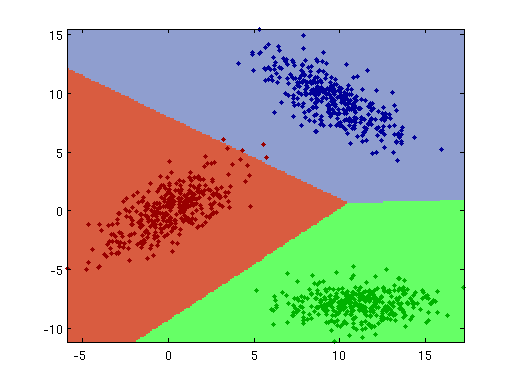
\includegraphics[clip, trim=40px 15px 30px 10px]{data1a_1a.png}
\caption{Bayes $C_{mean}$, Linearly separable data set}
\end{figure}
\begin{figure}[h]
\center
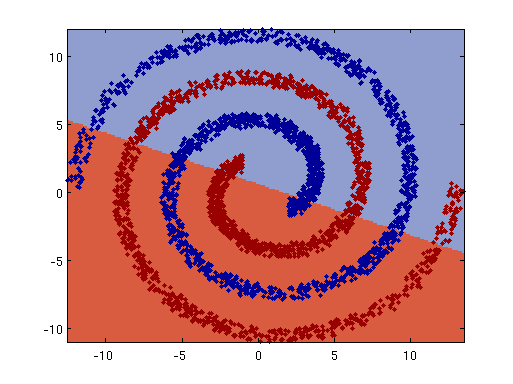
\includegraphics[clip, trim=40px 15px 30px 10px]{data1b_1a.png}
\caption{Bayes $C_{mean}$, Nonlinearly separable data set}
\end{figure}
\begin{figure}[h]
\center
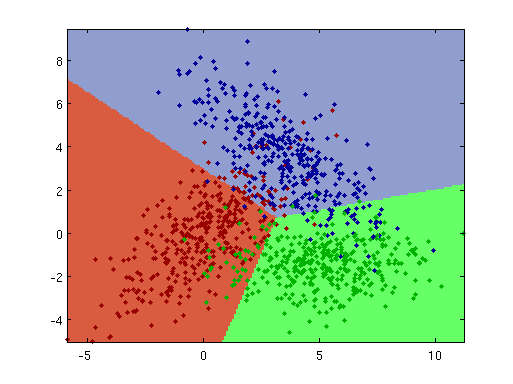
\includegraphics[clip, trim=40px 15px 30px 10px]{data1c_1a.png}
\caption{Bayes $C_{mean}$, Overlapping data set}
\end{figure}
\begin{figure}[h]
\center
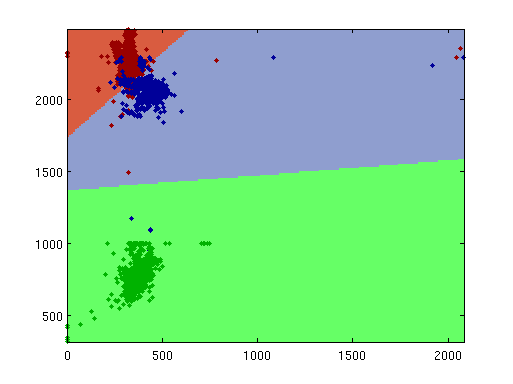
\includegraphics[clip, trim=40px 15px 30px 10px]{data2_1a.png}
\caption{Bayes $C_{mean}$, Real world data set}
\end{figure}
% Bayes C_distinct
\begin{figure}[h]
\center
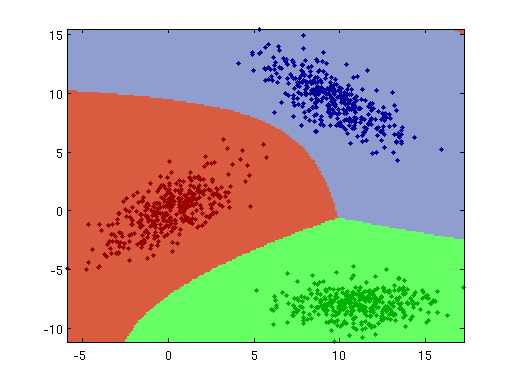
\includegraphics[clip, trim=40px 15px 30px 10px]{data1a_1b.png}
\caption{Bayes $C_{distinct}$, Linearly separable data set}
\end{figure}
\begin{figure}[h]
\center
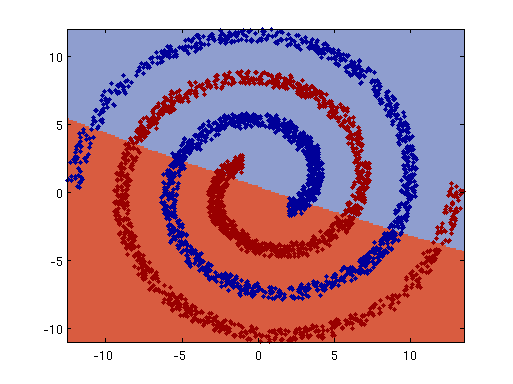
\includegraphics[clip, trim=40px 15px 30px 10px]{data1b_1b.png}
\caption{Bayes $C_{distinct}$, Nonlinearly separable data set}
\end{figure}
\begin{figure}[h]
\center
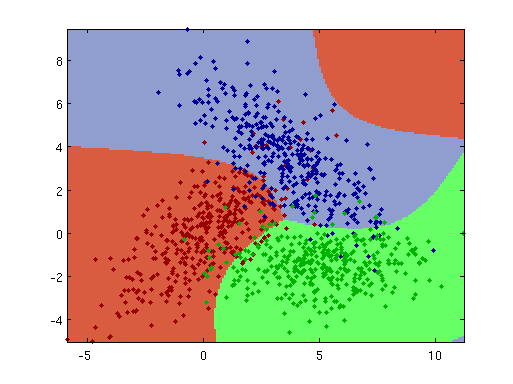
\includegraphics[clip, trim=40px 15px 30px 10px]{data1c_1b.png}
\caption{Bayes $C_{distinct}$, Overlapping data set}
\end{figure}
\begin{figure}[h]
\center
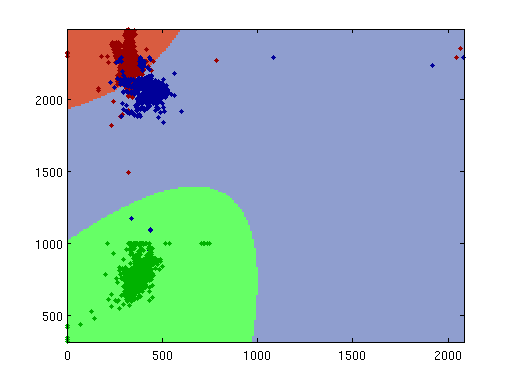
\includegraphics[clip, trim=40px 15px 30px 10px]{data2_1b.png}
\caption{Bayes $C_{distinct}$, Real world data set}
\end{figure}
% Naive Bayes C=\sigma^2 I
\begin{figure}[h]
\center
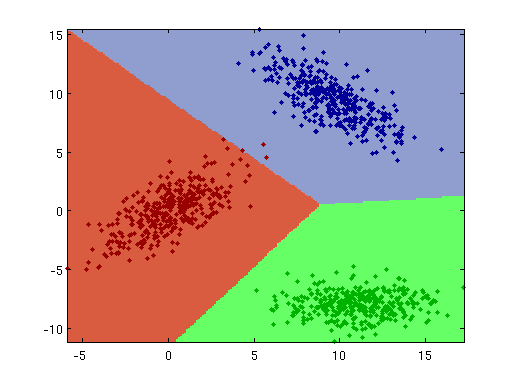
\includegraphics[clip, trim=40px 15px 30px 10px]{data1a_2a.png}
\caption{Naive Bayes $C = \sigma^2 I$, Linearly separable data set}
\end{figure}
\begin{figure}[h]
\center
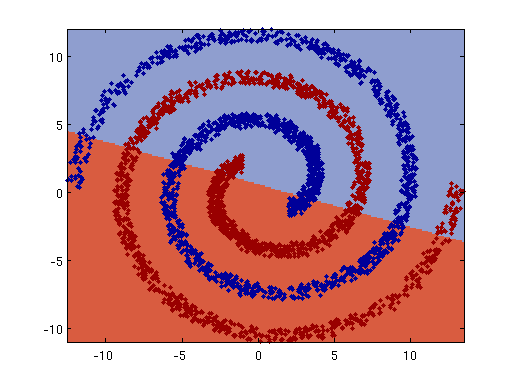
\includegraphics[clip, trim=40px 15px 30px 10px]{data1b_2a.png}
\caption{Naive Bayes $C = \sigma^2 I$, Nonlinearly separable data set}
\end{figure}
\begin{figure}[h]
\center
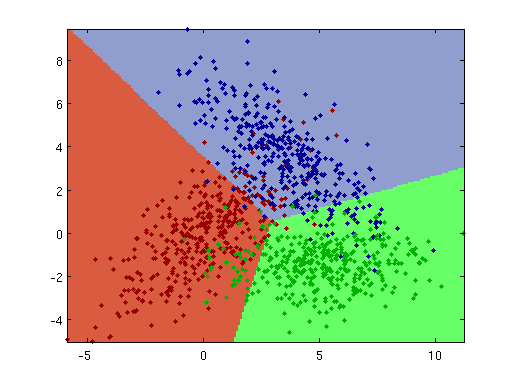
\includegraphics[clip, trim=40px 15px 30px 10px]{data1c_2a.png}
\caption{Naive Bayes $C = \sigma^2 I$, Overlapping data set}
\end{figure}
\begin{figure}[h]
\center
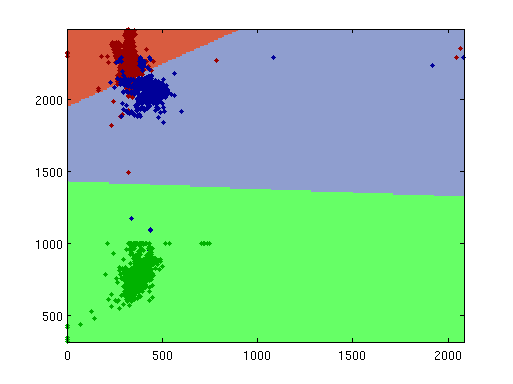
\includegraphics[clip, trim=40px 15px 30px 10px]{data2_2a.png}
\caption{Naive Bayes $C = \sigma^2 I$, Real world data set}
\end{figure}
\clearpage
% Naive Bayes C_mean
\begin{figure}[h]
\center
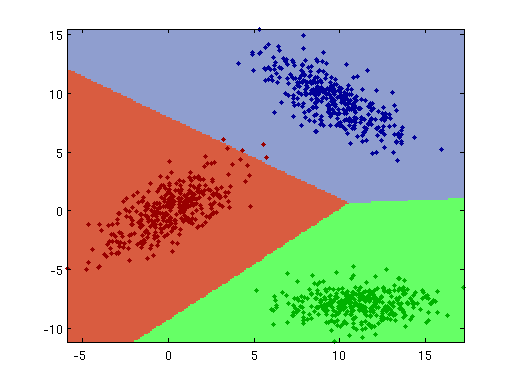
\includegraphics[clip, trim=40px 15px 30px 10px]{data1a_2b.png}
\caption{Naive Bayes $C_{mean}$, Linearly separable data set}
\end{figure}
\begin{figure}[h]
\center
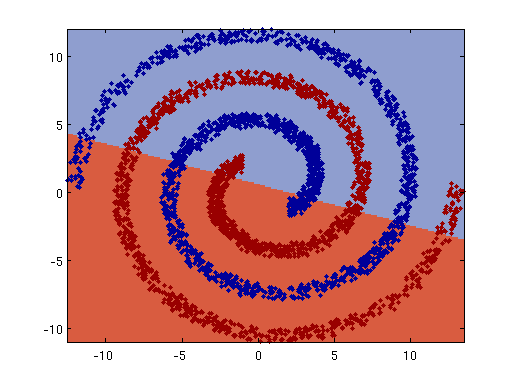
\includegraphics[clip, trim=40px 15px 30px 10px]{data1b_2b.png}
\caption{Naive Bayes $C_{mean}$, Noninearly separable data set}
\end{figure}
\begin{figure}[h]
\center
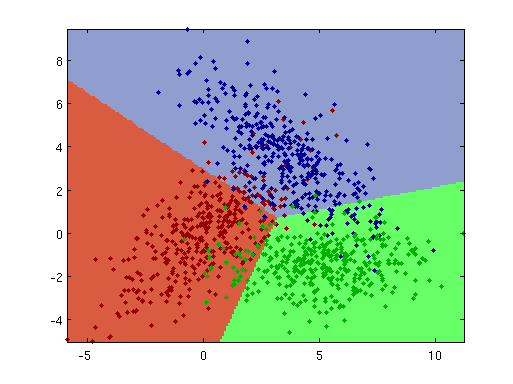
\includegraphics[clip, trim=40px 15px 30px 10px]{data1c_2b.png}
\caption{Naive Bayes $C_{mean}$, Overlapping data set}
\end{figure}
\begin{figure}[h]
\center
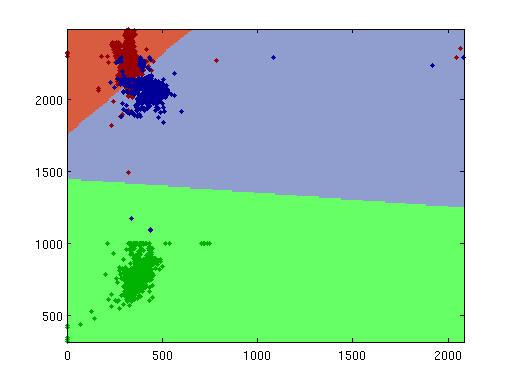
\includegraphics[clip, trim=40px 15px 30px 10px]{data2_2b.png}
\caption{Naive Bayes $C_{mean}$, Real world data set}
\end{figure}
% Naive Bayes C_distinct
\begin{figure}[h]
\center
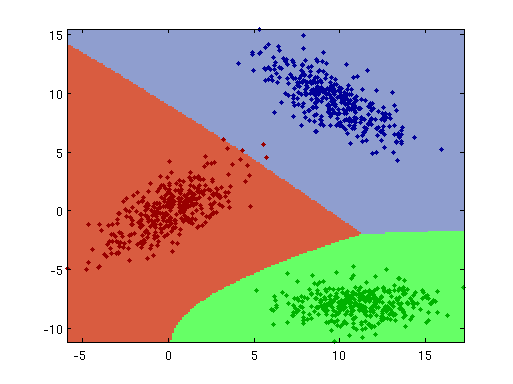
\includegraphics[clip, trim=40px 15px 30px 10px]{data1a_2c.png}
\caption{Naive Bayes $C_{distinct}$, Linearly separable data set}
\end{figure}
\begin{figure}[h]
\center
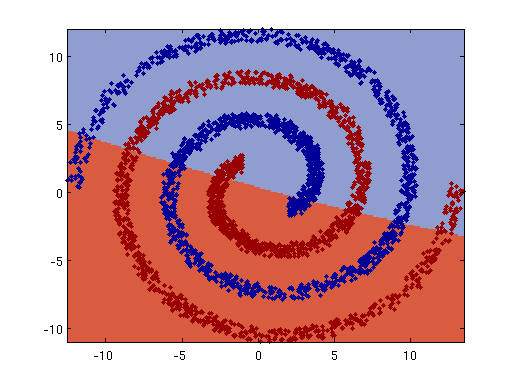
\includegraphics[clip, trim=40px 15px 30px 10px]{data1b_2c.png}
\caption{Naive Bayes $C_{distinct}$, Nonlinearly separable data set}
\end{figure}
\begin{figure}[h]
\center
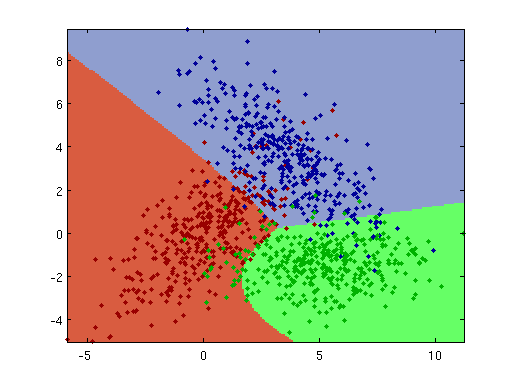
\includegraphics[clip, trim=40px 15px 30px 10px]{data1c_2c.png}
\caption{Naive Bayes $C_{distinct}$, Overlapping data set}
\end{figure}
\begin{figure}[h]
\center
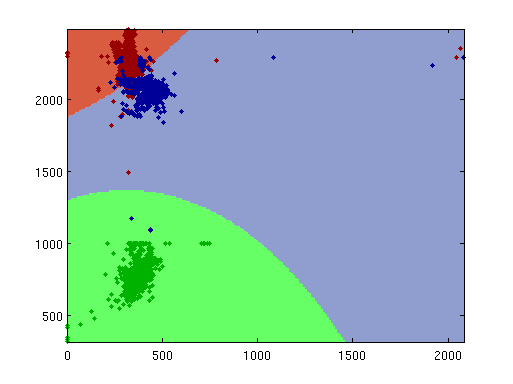
\includegraphics[clip, trim=40px 15px 30px 10px]{data2_2c.png}
\caption{Naive Bayes $C_{distinct}$, Real world data set}
\end{figure}
\end{document}

